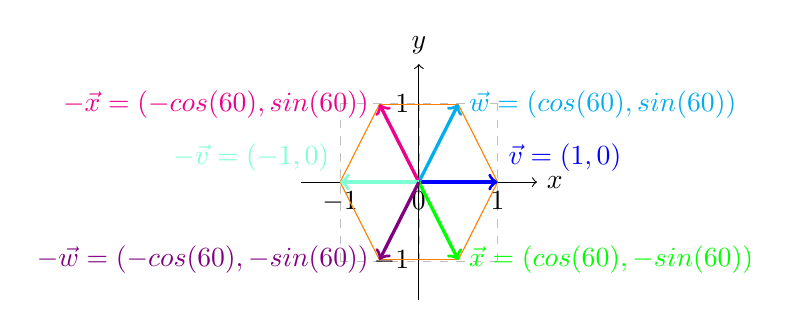
\begin{tikzpicture}
    \draw[step=1,help lines, dashed,lightgray] (-1,-1) grid (1,1);
    %draw axis value
    \foreach \x in {-1,0,1}
        {%
            \draw (\x,0) -- (\x,0) node [below] {$\x$};
        }
    \foreach \y in {-1,1}
        {%
            \draw (0,\y) -- (0,\y) node [left] {$\y$};
        }
    %draw lines
    \draw [->] (-1.5,0) -- (1.5,0) node[right]{$x$};
    \draw [->] (0,-1.5) -- (0,1.5) node[above]{$y$};
    \draw [-,orange] (1,0) -- (0.5,\fpeval{sin(-30)});
    \draw [-,orange] (0.5,\fpeval{sin(-30)}) -- (-0.5,\fpeval{sin(-30)});
    \draw [-,orange] (-0.5,\fpeval{sin(-30)}) -- (-1,0);
    \draw [-,orange] (-1,0) -- (-0.5,-\fpeval{sin(-30)});
    \draw [-,orange] (-0.5,-\fpeval{sin(-30)}) -- (0.5,-\fpeval{sin(-30)});
    \draw [-,orange] (0.5,-\fpeval{sin(-30)}) -- (1,0);
    \draw [->,blue,very thick] (0,0) -- (1,0) node[above right]{$\vec{v}=(1,0)$};
    \draw [->,cyan,very thick] (0,0) -- (0.5,\fpeval{sin(-30)}) node[right]{$\vec{w}=(cos(60),sin(60))$};
    \draw [->,green,very thick] (0,0) -- (0.5,\fpeval{-sin(-30)}) node[right]{$\vec{x}=(cos(60),-sin(60))$};
    \draw [->,magenta,very thick] (0,0) -- (-0.5,\fpeval{sin(-30)}) node[left]{$-\vec{x}=(-cos(60),sin(60))$};
    \draw [->,Aquamarine,very thick] (0,0) -- (-1,0) node[above left]{$-\vec{v}=(-1,0)$};
    \draw [->,violet,very thick] (0,0) -- (-0.5,\fpeval{-sin(-30)}) node[left]{$-\vec{w}=(-cos(60),-sin(60))$};
\end{tikzpicture}
\captionof{figure}{{\footnotesize vector to corners of hexagon}}
\label{fig:vector-and-vector-operation-d11}
